% Options for packages loaded elsewhere
\PassOptionsToPackage{unicode}{hyperref}
\PassOptionsToPackage{hyphens}{url}
%
\documentclass[
  10pt,
  ignorenonframetext,
]{beamer}
\usepackage{pgfpages}
\setbeamertemplate{caption}[numbered]
\setbeamertemplate{caption label separator}{: }
\setbeamercolor{caption name}{fg=normal text.fg}
\beamertemplatenavigationsymbolsempty
% Prevent slide breaks in the middle of a paragraph
\widowpenalties 1 10000
\raggedbottom
\setbeamertemplate{part page}{
  \centering
  \begin{beamercolorbox}[sep=16pt,center]{part title}
    \usebeamerfont{part title}\insertpart\par
  \end{beamercolorbox}
}
\setbeamertemplate{section page}{
  \centering
  \begin{beamercolorbox}[sep=12pt,center]{part title}
    \usebeamerfont{section title}\insertsection\par
  \end{beamercolorbox}
}
\setbeamertemplate{subsection page}{
  \centering
  \begin{beamercolorbox}[sep=8pt,center]{part title}
    \usebeamerfont{subsection title}\insertsubsection\par
  \end{beamercolorbox}
}
\AtBeginPart{
  \frame{\partpage}
}
\AtBeginSection{
  \ifbibliography
  \else
    \frame{\sectionpage}
  \fi
}
\AtBeginSubsection{
  \frame{\subsectionpage}
}

\usepackage{amsmath,amssymb}
\usepackage{iftex}
\ifPDFTeX
  \usepackage[T1]{fontenc}
  \usepackage[utf8]{inputenc}
  \usepackage{textcomp} % provide euro and other symbols
\else % if luatex or xetex
  \usepackage{unicode-math}
  \defaultfontfeatures{Scale=MatchLowercase}
  \defaultfontfeatures[\rmfamily]{Ligatures=TeX,Scale=1}
\fi
\usepackage{lmodern}
\ifPDFTeX\else  
    % xetex/luatex font selection
\fi
% Use upquote if available, for straight quotes in verbatim environments
\IfFileExists{upquote.sty}{\usepackage{upquote}}{}
\IfFileExists{microtype.sty}{% use microtype if available
  \usepackage[]{microtype}
  \UseMicrotypeSet[protrusion]{basicmath} % disable protrusion for tt fonts
}{}
\makeatletter
\@ifundefined{KOMAClassName}{% if non-KOMA class
  \IfFileExists{parskip.sty}{%
    \usepackage{parskip}
  }{% else
    \setlength{\parindent}{0pt}
    \setlength{\parskip}{6pt plus 2pt minus 1pt}}
}{% if KOMA class
  \KOMAoptions{parskip=half}}
\makeatother
\usepackage{xcolor}
\newif\ifbibliography
\setlength{\emergencystretch}{3em} % prevent overfull lines
\setcounter{secnumdepth}{-\maxdimen} % remove section numbering

\usepackage{color}
\usepackage{fancyvrb}
\newcommand{\VerbBar}{|}
\newcommand{\VERB}{\Verb[commandchars=\\\{\}]}
\DefineVerbatimEnvironment{Highlighting}{Verbatim}{commandchars=\\\{\}}
% Add ',fontsize=\small' for more characters per line
\usepackage{framed}
\definecolor{shadecolor}{RGB}{241,243,245}
\newenvironment{Shaded}{\begin{snugshade}}{\end{snugshade}}
\newcommand{\AlertTok}[1]{\textcolor[rgb]{0.68,0.00,0.00}{#1}}
\newcommand{\AnnotationTok}[1]{\textcolor[rgb]{0.37,0.37,0.37}{#1}}
\newcommand{\AttributeTok}[1]{\textcolor[rgb]{0.40,0.45,0.13}{#1}}
\newcommand{\BaseNTok}[1]{\textcolor[rgb]{0.68,0.00,0.00}{#1}}
\newcommand{\BuiltInTok}[1]{\textcolor[rgb]{0.00,0.23,0.31}{#1}}
\newcommand{\CharTok}[1]{\textcolor[rgb]{0.13,0.47,0.30}{#1}}
\newcommand{\CommentTok}[1]{\textcolor[rgb]{0.37,0.37,0.37}{#1}}
\newcommand{\CommentVarTok}[1]{\textcolor[rgb]{0.37,0.37,0.37}{\textit{#1}}}
\newcommand{\ConstantTok}[1]{\textcolor[rgb]{0.56,0.35,0.01}{#1}}
\newcommand{\ControlFlowTok}[1]{\textcolor[rgb]{0.00,0.23,0.31}{\textbf{#1}}}
\newcommand{\DataTypeTok}[1]{\textcolor[rgb]{0.68,0.00,0.00}{#1}}
\newcommand{\DecValTok}[1]{\textcolor[rgb]{0.68,0.00,0.00}{#1}}
\newcommand{\DocumentationTok}[1]{\textcolor[rgb]{0.37,0.37,0.37}{\textit{#1}}}
\newcommand{\ErrorTok}[1]{\textcolor[rgb]{0.68,0.00,0.00}{#1}}
\newcommand{\ExtensionTok}[1]{\textcolor[rgb]{0.00,0.23,0.31}{#1}}
\newcommand{\FloatTok}[1]{\textcolor[rgb]{0.68,0.00,0.00}{#1}}
\newcommand{\FunctionTok}[1]{\textcolor[rgb]{0.28,0.35,0.67}{#1}}
\newcommand{\ImportTok}[1]{\textcolor[rgb]{0.00,0.46,0.62}{#1}}
\newcommand{\InformationTok}[1]{\textcolor[rgb]{0.37,0.37,0.37}{#1}}
\newcommand{\KeywordTok}[1]{\textcolor[rgb]{0.00,0.23,0.31}{\textbf{#1}}}
\newcommand{\NormalTok}[1]{\textcolor[rgb]{0.00,0.23,0.31}{#1}}
\newcommand{\OperatorTok}[1]{\textcolor[rgb]{0.37,0.37,0.37}{#1}}
\newcommand{\OtherTok}[1]{\textcolor[rgb]{0.00,0.23,0.31}{#1}}
\newcommand{\PreprocessorTok}[1]{\textcolor[rgb]{0.68,0.00,0.00}{#1}}
\newcommand{\RegionMarkerTok}[1]{\textcolor[rgb]{0.00,0.23,0.31}{#1}}
\newcommand{\SpecialCharTok}[1]{\textcolor[rgb]{0.37,0.37,0.37}{#1}}
\newcommand{\SpecialStringTok}[1]{\textcolor[rgb]{0.13,0.47,0.30}{#1}}
\newcommand{\StringTok}[1]{\textcolor[rgb]{0.13,0.47,0.30}{#1}}
\newcommand{\VariableTok}[1]{\textcolor[rgb]{0.07,0.07,0.07}{#1}}
\newcommand{\VerbatimStringTok}[1]{\textcolor[rgb]{0.13,0.47,0.30}{#1}}
\newcommand{\WarningTok}[1]{\textcolor[rgb]{0.37,0.37,0.37}{\textit{#1}}}

\providecommand{\tightlist}{%
  \setlength{\itemsep}{0pt}\setlength{\parskip}{0pt}}\usepackage{longtable,booktabs,array}
\usepackage{calc} % for calculating minipage widths
\usepackage{caption}
% Make caption package work with longtable
\makeatletter
\def\fnum@table{\tablename~\thetable}
\makeatother
\usepackage{graphicx}
\makeatletter
\def\maxwidth{\ifdim\Gin@nat@width>\linewidth\linewidth\else\Gin@nat@width\fi}
\def\maxheight{\ifdim\Gin@nat@height>\textheight\textheight\else\Gin@nat@height\fi}
\makeatother
% Scale images if necessary, so that they will not overflow the page
% margins by default, and it is still possible to overwrite the defaults
% using explicit options in \includegraphics[width, height, ...]{}
\setkeys{Gin}{width=\maxwidth,height=\maxheight,keepaspectratio}
% Set default figure placement to htbp
\makeatletter
\def\fps@figure{htbp}
\makeatother

\linespread{1.15}
\usepackage{xcolor} % load xcolor for color commands
\setbeamertemplate{itemize item}{\raise0.5pt\hbox{\textcolor{black}{$\bullet$}}}
\setbeamerfont{frametitle}{size=\large}
\usepackage{etoolbox}
\AtBeginEnvironment{verbatim}{\setlength{\parskip}{0pt}\setlength{\topsep}{0pt}}
\makeatletter
\@ifpackageloaded{caption}{}{\usepackage{caption}}
\AtBeginDocument{%
\ifdefined\contentsname
  \renewcommand*\contentsname{Table of contents}
\else
  \newcommand\contentsname{Table of contents}
\fi
\ifdefined\listfigurename
  \renewcommand*\listfigurename{List of Figures}
\else
  \newcommand\listfigurename{List of Figures}
\fi
\ifdefined\listtablename
  \renewcommand*\listtablename{List of Tables}
\else
  \newcommand\listtablename{List of Tables}
\fi
\ifdefined\figurename
  \renewcommand*\figurename{Figure}
\else
  \newcommand\figurename{Figure}
\fi
\ifdefined\tablename
  \renewcommand*\tablename{Table}
\else
  \newcommand\tablename{Table}
\fi
}
\@ifpackageloaded{float}{}{\usepackage{float}}
\floatstyle{ruled}
\@ifundefined{c@chapter}{\newfloat{codelisting}{h}{lop}}{\newfloat{codelisting}{h}{lop}[chapter]}
\floatname{codelisting}{Listing}
\newcommand*\listoflistings{\listof{codelisting}{List of Listings}}
\makeatother
\makeatletter
\makeatother
\makeatletter
\@ifpackageloaded{caption}{}{\usepackage{caption}}
\@ifpackageloaded{subcaption}{}{\usepackage{subcaption}}
\makeatother

\ifLuaTeX
  \usepackage{selnolig}  % disable illegal ligatures
\fi
\usepackage{bookmark}

\IfFileExists{xurl.sty}{\usepackage{xurl}}{} % add URL line breaks if available
\urlstyle{same} % disable monospaced font for URLs
\hypersetup{
  pdftitle={Logistic Regression in R + Quarto Docs},
  pdfauthor={Matthias Frühwirth},
  hidelinks,
  pdfcreator={LaTeX via pandoc}}


\title{Logistic Regression in R + Quarto Docs}
\subtitle{\href{./index.html}{Data Literacy}}
\author{Matthias Frühwirth}
\date{}
\institute{\href{https://www.wu.ac.at/retail/}{Institute for Retailing
\& Data Science}}

\begin{document}
\frame{\titlepage}


\begin{frame}{Recap and Intro}
\phantomsection\label{recap-and-intro}
Last week

\begin{itemize}
\tightlist
\item
  Causal Inference
\item
  DAGs \& Diff-in-Diff
\item
  Quarto Presentations
\end{itemize}

Today

\begin{itemize}
\tightlist
\item
  Logistic Regression
\item
  Quarto Documents
\end{itemize}
\end{frame}

\begin{frame}{Intro to Logistic Regression (Logit)}
\phantomsection\label{intro-to-logistic-regression-logit}
Logistic Regression

\begin{itemize}
\item
  Can be used if outcome is a binary variable (e.g.~1 = Purchase
  Complete, 0 = Cart Abandoned)
\item
  Generalized Linear Model (linear regression + non-linear link
  function, marginal effects are non-linear)
\item
  Interested in modelling probabilities of outcomes:

  Q: \emph{``How does making payment one-click affect the probability
  that the purchase is completed''? What about browsing time on the
  website?}
\item
  Sits right at the intersection of econometrics and machine learning
\item
  Widely used baseline for inference, prediction/classification with
  category outcomes
\end{itemize}
\end{frame}

\begin{frame}{Graphical}
\phantomsection\label{graphical}
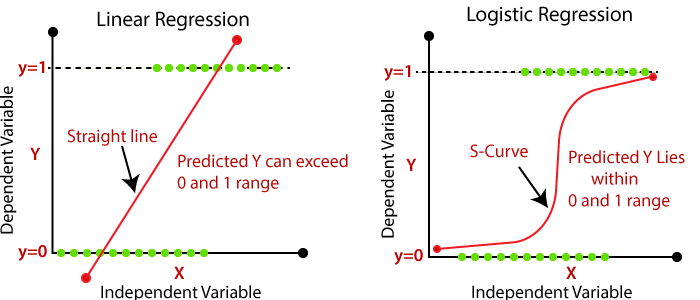
\includegraphics[width=3.64583in,height=\textheight]{images/linear-regression-vs-logistic-regression.png}

As we change X, we change the probability that Y becomes 1.
\end{frame}

\begin{frame}{Basics}
\phantomsection\label{basics}
\begin{itemize}
\item
  We assume that the outcome is Bernoulli distributed (outcome of a
  Bernoulli trial): this means with probability \(p\) the outcome is 1
  and with probability \(1-p\) it is 0.
\item
  We are interested in \(p\), so logistic regression models the
  probability of a binary outcome (Y = 0, 1). Probability Form:
\end{itemize}

\[
  P(Y = 1 \mid X) = \frac{1}{1 + e^{-\textcolor{blue}{\beta_0 + \beta_1 X_1 + \dots + \beta_k X_k}}}
\]

\begin{itemize}
\tightlist
\item
  Equivalent log odds form: The model assumes a \textbf{logit (log-odds)
  link} between predictors and the probability:
\end{itemize}

\[
\log\left(\frac{P(Y = 1 \mid X)}{1 - P(Y = 1 \mid X)}\right) = \textcolor{blue}{\beta_0 + \beta_1 X_1 + \dots + \beta_k X_k}
\]
\end{frame}

\begin{frame}{Odds and Interpretation}
\phantomsection\label{odds-and-interpretation}
\small

\begin{itemize}
\item
  We can interpret a coefficient \(\beta_k\) as changes to the log-odds;
  and \(\exp(\beta_k)\) as changes to odds. \[
  \log\left(\underbrace{\frac{P(Y = 1 \mid X)}{1 - P(Y = 1 \mid X)}}_{\text{Odds}}\right) = \beta_0 + \beta_1 X_1 + \dots + \beta_k X_k.
  \]
\item
  Odds reflect how likely an event is compared to it not happening
  (``ratio of 1 to 0''), rather than its share of all outcomes (which
  would be the probability).
\item
  \textbf{Example}: The baseline odds for 100 customers (20 purchase
  complete, 80 cart abandoned). Then you estimate \(\beta_k = 0.5\):
\end{itemize}

\[
  \text{Odds} = \frac{20}{80} = 0.25 \quad\quad e^{\beta_k = 0.5} \approx 1.65 \quad\quad \text{New Odds} = 0.25 \times 1.65 \approx 0.4125.
\]

\begin{itemize}
\tightlist
\item
  For a one-unit increase in \(\beta_k\), the odds increase by about
  \((\exp(\beta) - 1) \cdot 100 \% = 65\%\). However, the effect on the
  actual probability depends on the starting value of the regressors.
\end{itemize}
\end{frame}

\begin{frame}{Probabilites}
\phantomsection\label{probabilites}
\small

\begin{itemize}
\item
  Coefficients from the regression output can be directly interpreted as
  changes to (log-)odds. If \(\beta_1\) \textgreater{} 0, odds increase,
  as well as probabilities (and reverse). The change does not depend on
  the actual level of X.
\item
  The reason: Odds are multiplicative, log-odds are additive (changes
  are ``just added'').
\item
  However, the change in the outcome probability P(\(Y = 1 \mid X\))
  depends on the starting level of the covariates.
\item
  Also note: \[
  P(Y = 1) = \frac{\text{Odds}}{1 + \text{Odds}}
  \]
\item
  Previous Example (odds before: \(0.25\), odds after: \(0.41\))
\end{itemize}

\[
p_{\text{1}} = \frac{20}{20+80} = \frac{0.25}{1 + 1.25} = 0.2, \quad  p_{\text{new}} \approx \frac{0.4125}{1.4125} \approx 0.291.
\]

\begin{itemize}
\tightlist
\item
  Interpretation: For the given baseline probability/odds, increasing
  the explanatory variable by one unit increases the probability of
  \(Y\) by approx. \(9.1\%\).
\end{itemize}
\end{frame}

\begin{frame}[fragile]{How to do in R:}
\phantomsection\label{how-to-do-in-r}
\footnotesize

\begin{itemize}
\tightlist
\item
  Use the \texttt{glm} (generalized linear models) function from base R.
\end{itemize}

\begin{Shaded}
\begin{Highlighting}[]
\NormalTok{logit\_model }\OtherTok{\textless{}{-}} \FunctionTok{glm}\NormalTok{(Y }\SpecialCharTok{\textasciitilde{}}\NormalTok{ X1 }\SpecialCharTok{+}\NormalTok{ X2, }\AttributeTok{data =}\NormalTok{ df, }\AttributeTok{family =}\NormalTok{ binomial)}
\FunctionTok{summary}\NormalTok{(logit\_model)}
\end{Highlighting}
\end{Shaded}

\begin{itemize}
\tightlist
\item
  Model Fit (Pseudo-\(R^2\)):
\end{itemize}

\begin{Shaded}
\begin{Highlighting}[]
\NormalTok{pscl}\SpecialCharTok{::}\FunctionTok{pR2}\NormalTok{(logit\_model)}
\end{Highlighting}
\end{Shaded}

\begin{itemize}
\tightlist
\item
  Calculate predicted probabilities:
\end{itemize}

\begin{Shaded}
\begin{Highlighting}[]
\FunctionTok{predict}\NormalTok{(logit\_model, }\AttributeTok{type =} \StringTok{"response"}\NormalTok{)}
\end{Highlighting}
\end{Shaded}

\begin{itemize}
\tightlist
\item
  Get changes in probabilities (average marginal effects, keeps other
  covariates constant for each obs.)
\end{itemize}

\begin{Shaded}
\begin{Highlighting}[]
\CommentTok{\#install.packages("margins")}
\FunctionTok{library}\NormalTok{(margins)}
\NormalTok{marginal\_effects }\OtherTok{\textless{}{-}} \FunctionTok{margins}\NormalTok{(logit\_model)}
\FunctionTok{summary}\NormalTok{(marginal\_effects)}
\end{Highlighting}
\end{Shaded}
\end{frame}

\begin{frame}{Example Logit: Movie Box-Office-Bombs}
\phantomsection\label{example-logit-movie-box-office-bombs}
\small

\begin{itemize}
\item
  1812 movies released in U.S. cinemas between 1995 and 2024 with a
  budget of at least 25 million dollars.
\item
  We are interested in if a film is a box office flop (``bomb'').
  Defined as ROI \textless{} 66\% and no international success
  \(\rightarrow\) Y = 1 (is a bomb).
\item
  Explanatory variables (in the data) are audience and critical scores,
  as well as film properties like runtime and genre.
\item
  Source: BoxOfficeMojo + IMDb + RottenTomatoes
\end{itemize}

\begin{columns}[T]
\begin{column}{0.48\textwidth}
\centering


\includegraphics[width=1.04167in,height=\textheight]{images/MV5BZWNmZGYzZjUtODRmOS00ODgzLWE4NWQtMDI3MGUwNjRjYjY0XkEyXkFqcGc@._V1_FMjpg_UX1000_.jpg}
\end{column}

\begin{column}{0.48\textwidth}
\scriptsize

\textbf{John Carter (2012)}

\begin{itemize}
\tightlist
\item
  Budget: 250 million USD\\
\item
  Domestic Box Office: 73 million USD\\
\item
  Audience Score: 60 \& Critic Score: 52 (RT), runtime: 132 minutes\\
\item
  One of the biggest bombs of all time (Disney took a 200 million dollar
  write-off)
\end{itemize}
\end{column}
\end{columns}
\end{frame}

\begin{frame}[fragile]{Data}
\phantomsection\label{data}
\scriptsize

\begin{Shaded}
\begin{Highlighting}[]
\NormalTok{df\_movie }\OtherTok{\textless{}{-}} \FunctionTok{read\_csv}\NormalTok{(}\StringTok{"movie\_select.csv"}\NormalTok{) }

\NormalTok{df\_movie }\SpecialCharTok{\%\textgreater{}\%} 
  \FunctionTok{select}\NormalTok{(title,budget, domestic,runtime,audience\_score,critic\_score,is\_bo\_bomb) }\SpecialCharTok{\%\textgreater{}\%} 
  \FunctionTok{arrange}\NormalTok{(}\SpecialCharTok{{-}}\NormalTok{budget) }\SpecialCharTok{\%\textgreater{}\%} \FunctionTok{head}\NormalTok{(}\DecValTok{7}\NormalTok{)}
\end{Highlighting}
\end{Shaded}

\begin{verbatim}
# A tibble: 7 x 7
  title           budget domestic runtime audience_score critic_score is_bo_bomb
  <chr>            <dbl>    <dbl>   <dbl>          <dbl>        <dbl>      <dbl>
1 Indiana Jones ~    387      174     154             88           70          1
2 Avengers: Endg~    356      858     181             90           94          0
3 Fast X(2023)       340      146     141             84           56          0
4 Avengers: Infi~    321      678     149             92           85          0
5 Pirates of the~    300      309     169             72           44          0
6 Mission: Impos~    291      172     163             94           96          0
7 Solo: A Star W~    275      213     135             63           69          0
\end{verbatim}
\end{frame}

\begin{frame}{Distributions}
\phantomsection\label{distributions}
\begin{center}
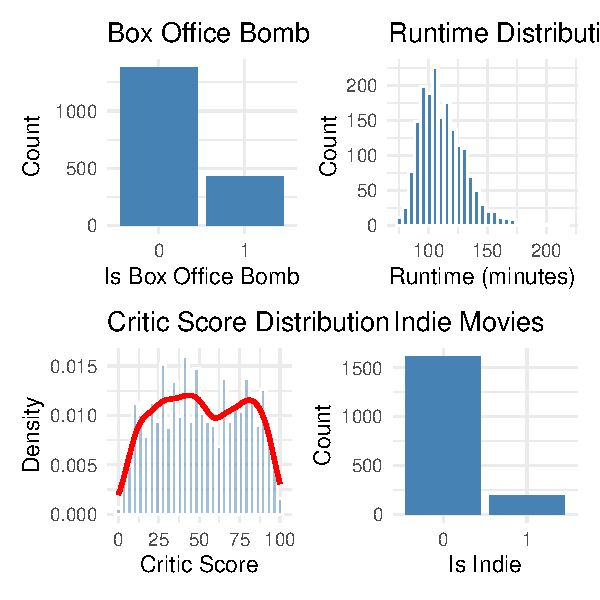
\includegraphics[width=0.7\textwidth,height=\textheight]{logit_files/figure-beamer/unnamed-chunk-6-1.pdf}
\end{center}
\end{frame}

\begin{frame}[fragile]{Estimate Model}
\phantomsection\label{estimate-model}
\scriptsize

\begin{Shaded}
\begin{Highlighting}[]
\NormalTok{logit\_model }\OtherTok{\textless{}{-}} \FunctionTok{glm}\NormalTok{(is\_bo\_bomb }\SpecialCharTok{\textasciitilde{}}\NormalTok{  runtime }\SpecialCharTok{+}\NormalTok{ imdb\_avg\_rating }\SpecialCharTok{+} 
\NormalTok{                     audience\_score }\SpecialCharTok{+}\NormalTok{ critic\_score }\SpecialCharTok{+}\NormalTok{ is\_indie }\SpecialCharTok{+} 
\NormalTok{                     ge\_action }\SpecialCharTok{+}\NormalTok{ ge\_animation, }\CommentTok{\#+ factor(title\_year),}
                   \AttributeTok{data =}\NormalTok{ df\_movie,}
                   \AttributeTok{family =}\NormalTok{ binomial)}

\NormalTok{pscl}\SpecialCharTok{::}\FunctionTok{pR2}\NormalTok{(logit\_model) }\CommentTok{\# Print R2 (McFadden) + eval}
\end{Highlighting}
\end{Shaded}

\begin{verbatim}
fitting null model for pseudo-r2
\end{verbatim}

\begin{verbatim}
         llh      llhNull           G2     McFadden         r2ML         r2CU 
-888.6360852 -995.2245458  213.1769211    0.1070999    0.1109905    0.1664965 
\end{verbatim}
\end{frame}

\begin{frame}[fragile]{Model Summary}
\phantomsection\label{model-summary}
\tiny

\begin{Shaded}
\begin{Highlighting}[]
\FunctionTok{summary}\NormalTok{(logit\_model) }\CommentTok{\# Print summary}
\end{Highlighting}
\end{Shaded}

\begin{verbatim}

Call:
glm(formula = is_bo_bomb ~ runtime + imdb_avg_rating + audience_score + 
    critic_score + is_indie + ge_action + ge_animation, family = binomial, 
    data = df_movie)

Deviance Residuals: 
    Min       1Q   Median       3Q      Max  
-1.6731  -0.7543  -0.5323  -0.2811   2.8183  

Coefficients:
                 Estimate Std. Error z value   Pr(>|z|)    
(Intercept)      1.470635   0.543181   2.707   0.006780 ** 
runtime          0.010314   0.003738   2.759   0.005799 ** 
imdb_avg_rating -0.346688   0.116730  -2.970   0.002978 ** 
audience_score  -0.018976   0.005279  -3.595   0.000325 ***
critic_score    -0.009036   0.003473  -2.602   0.009272 ** 
is_indie         0.820175   0.168235   4.875 0.00000109 ***
ge_action       -0.524517   0.124737  -4.205 0.00002611 ***
ge_animation    -0.402121   0.265862  -1.513   0.130401    
---
Signif. codes:  0 '***' 0.001 '**' 0.01 '*' 0.05 '.' 0.1 ' ' 1

(Dispersion parameter for binomial family taken to be 1)

    Null deviance: 1990.4  on 1811  degrees of freedom
Residual deviance: 1777.3  on 1804  degrees of freedom
AIC: 1793.3

Number of Fisher Scoring iterations: 4
\end{verbatim}
\end{frame}

\begin{frame}{Interpreting Coefficients (Odds)}
\phantomsection\label{interpreting-coefficients-odds}
\scriptsize

\begin{itemize}
\item
  \textbf{Runtime (Estimate = 0.0103):}\\
  For each additional minute of runtime, the log-odds of being a box
  office bomb increase by 0.0103. This corresponds to an odds ratio of
  \(\exp(0.0103) \approx 1.01,\) meaning about a \textbf{1\% increase}
  in the odds per minute.
\item
  \textbf{Audience Score (Estimate = -0.0189):}\\
  Each one-point increase in the RT audience score decreases the
  log-odds by 0.019. This also implies implies a \textbf{(exp(-0.018976)
  - 1)*100\% = -1.879\% change} (decrease) in the odds of being a box
  office bomb per point.
\item
  \textbf{Is Indie (Estimate = 0.8201):}\\
  Being an indie film (when (\text{is\_indie} = 1)) increases the
  log-odds by 0.82 relative to non-indie films. This translates to an
  odds ratio of an odds ratio of 2.27, indicating that indie films have
  approximately \textbf{127\% higher odds} of being a box office bomb
  compared to non-indie films.
\end{itemize}
\end{frame}

\begin{frame}[fragile]{Marginal Effects (on P(Y = 1))}
\phantomsection\label{marginal-effects-on-py-1}
\scriptsize

\begin{Shaded}
\begin{Highlighting}[]
\NormalTok{marginal\_effects }\OtherTok{\textless{}{-}} \FunctionTok{margins}\NormalTok{(logit\_model)}
\FunctionTok{summary}\NormalTok{(marginal\_effects)}
\end{Highlighting}
\end{Shaded}

\begin{verbatim}
          factor     AME     SE       z      p   lower   upper
  audience_score -0.0030 0.0008 -3.6310 0.0003 -0.0047 -0.0014
    critic_score -0.0014 0.0006 -2.6134 0.0090 -0.0025 -0.0004
       ge_action -0.0840 0.0197 -4.2652 0.0000 -0.1226 -0.0454
    ge_animation -0.0644 0.0425 -1.5140 0.1300 -0.1477  0.0190
 imdb_avg_rating -0.0555 0.0185 -2.9953 0.0027 -0.0918 -0.0192
        is_indie  0.1313 0.0263  4.9858 0.0000  0.0797  0.1829
         runtime  0.0017 0.0006  2.7765 0.0055  0.0005  0.0028
\end{verbatim}

Interpretation. On average:

\begin{itemize}
\item
  a one-unit decrease in the audience score decreases the probability
  that the film is a box office bomb by 0.3\%.
\item
  a one-unit increase in the runtime increases the probability that the
  film is a box office bomb by 0.17\%.
\item
  switching from a non-indie to an indie film increases the predicted
  probability by roughly 13.1 {[}7.9, 18.2{]} percentage points.
\end{itemize}
\end{frame}

\begin{frame}[fragile]{Prediction: Predict/classify new data}
\phantomsection\label{prediction-predictclassify-new-data}
\scriptsize

\textbf{Create a stinker (long and bad reviews)}

\begin{Shaded}
\begin{Highlighting}[]
\NormalTok{new\_bad\_film }\OtherTok{\textless{}{-}} \FunctionTok{data.frame}\NormalTok{(}
  \AttributeTok{runtime =} \DecValTok{240}\NormalTok{,  }
  \AttributeTok{imdb\_avg\_rating =} \FloatTok{6.2}\NormalTok{, }\AttributeTok{audience\_score =} \DecValTok{22}\NormalTok{, }\AttributeTok{critic\_score =} \DecValTok{34}\NormalTok{,    }\CommentTok{\# BAD REVIEWS!}
  \AttributeTok{is\_indie =} \DecValTok{1}\NormalTok{, }\AttributeTok{ge\_action =} \DecValTok{0}\NormalTok{, }\AttributeTok{ge\_animation =} \DecValTok{0}
\NormalTok{)}

\NormalTok{predicted\_prob }\OtherTok{\textless{}{-}} \FunctionTok{predict}\NormalTok{(logit\_model, }\AttributeTok{newdata =}\NormalTok{ new\_bad\_film, }\AttributeTok{type =} \StringTok{"response"}\NormalTok{)}
\FunctionTok{cat}\NormalTok{(}\StringTok{"The probability of bombing is: "}\NormalTok{, predicted\_prob)}
\end{Highlighting}
\end{Shaded}

\begin{verbatim}
The probability of bombing is:  0.868991
\end{verbatim}

\textbf{Create a masterpiece (great reviews and not too long)}

\begin{Shaded}
\begin{Highlighting}[]
\NormalTok{new\_great\_film }\OtherTok{\textless{}{-}} \FunctionTok{data.frame}\NormalTok{(}
  \AttributeTok{runtime =} \DecValTok{120}\NormalTok{,  }
  \AttributeTok{imdb\_avg\_rating =} \FloatTok{9.2}\NormalTok{, }\AttributeTok{audience\_score =} \DecValTok{89}\NormalTok{, }\AttributeTok{critic\_score =} \DecValTok{79}\NormalTok{,    }
  \AttributeTok{is\_indie =} \DecValTok{0}\NormalTok{, }\AttributeTok{ge\_action =} \DecValTok{0}\NormalTok{, }\AttributeTok{ge\_animation =} \DecValTok{1}
\NormalTok{)}

\NormalTok{predicted\_prob }\OtherTok{\textless{}{-}} \FunctionTok{predict}\NormalTok{(logit\_model, }\AttributeTok{newdata =}\NormalTok{ new\_great\_film, }\AttributeTok{type =} \StringTok{"response"}\NormalTok{)}
\FunctionTok{cat}\NormalTok{(}\StringTok{"The probability of bombing is: "}\NormalTok{, predicted\_prob)}
\end{Highlighting}
\end{Shaded}

\begin{verbatim}
The probability of bombing is:  0.03605312
\end{verbatim}
\end{frame}

\begin{frame}[fragile]{Prediction and Classification (on existing data)
and Model Eval}
\phantomsection\label{prediction-and-classification-on-existing-data-and-model-eval}
\scriptsize

\begin{itemize}
\item
  Since logit is a common classifier, we can also evaluate our model on
  the quality of the models predicition (not just probabilities)
\item
  We can compare actual classes to predicted classes and look at how
  often the model is wrong (``cross entropy loss'').
\end{itemize}

\textbf{Add the predicted probability as a new column and construct the
predicted class (threshold 0.5)}

\begin{Shaded}
\begin{Highlighting}[]
\FunctionTok{set.seed}\NormalTok{(}\DecValTok{100}\NormalTok{)}
\NormalTok{df\_movie }\OtherTok{\textless{}{-}}\NormalTok{ df\_movie }\SpecialCharTok{\%\textgreater{}\%}
  \FunctionTok{mutate}\NormalTok{(}
    \AttributeTok{predicted\_prob =} \FunctionTok{predict}\NormalTok{(logit\_model, }\AttributeTok{type =} \StringTok{"response"}\NormalTok{),}
    \AttributeTok{predicted\_class =} \FunctionTok{if\_else}\NormalTok{(predicted\_prob }\SpecialCharTok{\textgreater{}=} \FloatTok{0.5}\NormalTok{, }\DecValTok{1}\NormalTok{, }\DecValTok{0}\NormalTok{)}
\NormalTok{  )}

\NormalTok{df\_movie }\SpecialCharTok{\%\textgreater{}\%} \FunctionTok{select}\NormalTok{(title,is\_bo\_bomb,predicted\_prob,predicted\_class) }\SpecialCharTok{\%\textgreater{}\%} 
  \FunctionTok{slice\_sample}\NormalTok{(}\AttributeTok{n =} \DecValTok{6}\NormalTok{)}
\end{Highlighting}
\end{Shaded}

\begin{verbatim}
# A tibble: 6 x 4
  title                    is_bo_bomb predicted_prob predicted_class
  <chr>                         <dbl>          <dbl>           <dbl>
1 Mumford(1999)                     1         0.184                0
2 The Social Network(2010)          0         0.0749               0
3 Sanctum(2011)                     0         0.277                0
4 Lucky Numbers(2000)               1         0.554                1
5 Nanny McPhee(2005)                0         0.154                0
6 Barney's Version(2010)            1         0.135                0
\end{verbatim}
\end{frame}

\begin{frame}[fragile]{Confusion Matrix and Metrics (from package
yardstick)}
\phantomsection\label{confusion-matrix-and-metrics-from-package-yardstick}
\scriptsize

\begin{Shaded}
\begin{Highlighting}[]
\NormalTok{df\_movie }\OtherTok{\textless{}{-}}\NormalTok{ df\_movie }\SpecialCharTok{\%\textgreater{}\%}
  \FunctionTok{mutate}\NormalTok{(}
    \AttributeTok{truth =} \FunctionTok{factor}\NormalTok{(is\_bo\_bomb, }\AttributeTok{levels =} \FunctionTok{c}\NormalTok{(}\DecValTok{1}\NormalTok{, }\DecValTok{0}\NormalTok{), }\AttributeTok{labels =} \FunctionTok{c}\NormalTok{(}\StringTok{"Yes"}\NormalTok{, }\StringTok{"No"}\NormalTok{)),}
    \AttributeTok{predicted =} \FunctionTok{factor}\NormalTok{(predicted\_class, }\AttributeTok{levels =} \FunctionTok{c}\NormalTok{(}\DecValTok{1}\NormalTok{, }\DecValTok{0}\NormalTok{), }\AttributeTok{labels =} \FunctionTok{c}\NormalTok{(}\StringTok{"Yes"}\NormalTok{, }\StringTok{"No"}\NormalTok{))}
\NormalTok{  )}

\NormalTok{cm }\OtherTok{\textless{}{-}}\NormalTok{ yardstick}\SpecialCharTok{::}\FunctionTok{conf\_mat}\NormalTok{(df\_movie, truth, predicted)}
\end{Highlighting}
\end{Shaded}

\begin{columns}[T]
\begin{column}{0.48\textwidth}
\vspace{1.1cm}

\begin{verbatim}
          Truth
Prediction  Yes   No
       Yes   63   50
       No   369 1330
\end{verbatim}
\end{column}

\begin{column}{0.48\textwidth}
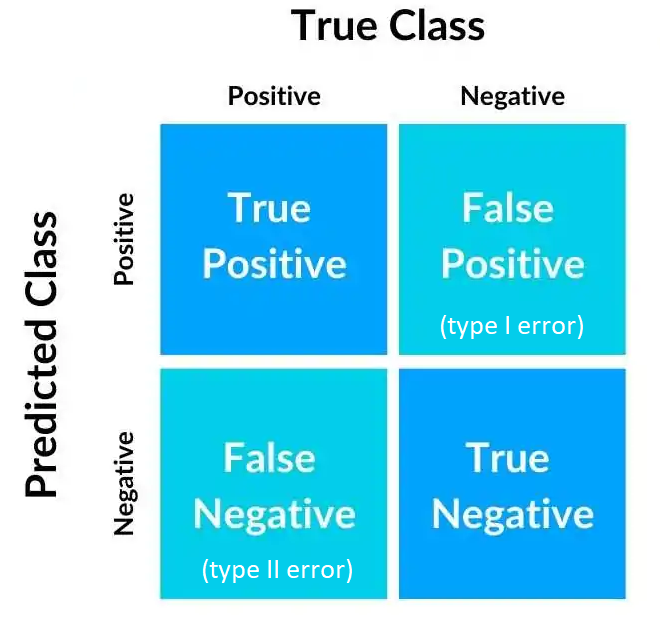
\includegraphics[width=1.5in,height=\textheight]{confusion_matrix.png}
\end{column}
\end{columns}
\end{frame}

\begin{frame}[fragile]{Metrics}
\phantomsection\label{metrics}
\scriptsize

There are several metrics than can be used to evaluate a binary
classification model (can also use yardstick functions), which depend on
these 4 values.

\begin{columns}[T]
\begin{column}{0.48\textwidth}
\begin{verbatim}
          Truth
Prediction  Yes   No
       Yes   63   50
       No   369 1330
\end{verbatim}
\end{column}

\begin{column}{0.48\textwidth}
\begin{Shaded}
\begin{Highlighting}[]
\NormalTok{TP }\OtherTok{\textless{}{-}} \DecValTok{63} \CommentTok{\# True positives}
\NormalTok{TN }\OtherTok{\textless{}{-}} \DecValTok{1330} \CommentTok{\# True negatives}
\NormalTok{FP }\OtherTok{\textless{}{-}} \DecValTok{50} \CommentTok{\# False positives}
\NormalTok{FN }\OtherTok{\textless{}{-}} \DecValTok{369} \CommentTok{\# False negatives}
\end{Highlighting}
\end{Shaded}
\end{column}
\end{columns}

\scriptsize

\begin{itemize}
\item
  Accuracy (overall correctness):

\begin{Shaded}
\begin{Highlighting}[]
\NormalTok{(TP }\SpecialCharTok{+}\NormalTok{ TN) }\SpecialCharTok{/}\NormalTok{ (TP }\SpecialCharTok{+}\NormalTok{ TN }\SpecialCharTok{+}\NormalTok{ FP }\SpecialCharTok{+}\NormalTok{ FN)}
\end{Highlighting}
\end{Shaded}

\begin{verbatim}
[1] 0.7687638
\end{verbatim}
\item
  Sensitivity/Recall: indicates how well the model identifies actual
  positives.

\begin{Shaded}
\begin{Highlighting}[]
\NormalTok{TP }\SpecialCharTok{/}\NormalTok{ (TP }\SpecialCharTok{+}\NormalTok{ FN)}
\end{Highlighting}
\end{Shaded}

\begin{verbatim}
[1] 0.1458333
\end{verbatim}
\item
  Specificity/True Negative Rate: measures how well the model identifies
  actual negatives.

\begin{Shaded}
\begin{Highlighting}[]
\NormalTok{TN }\SpecialCharTok{/}\NormalTok{ (TN }\SpecialCharTok{+}\NormalTok{ FP)}
\end{Highlighting}
\end{Shaded}

\begin{verbatim}
[1] 0.9637681
\end{verbatim}
\item
  Precision: reflects the accuracy of the positive predictions.

\begin{Shaded}
\begin{Highlighting}[]
\NormalTok{TP }\SpecialCharTok{/}\NormalTok{ (TP }\SpecialCharTok{+}\NormalTok{ FP)}
\end{Highlighting}
\end{Shaded}

\begin{verbatim}
[1] 0.5575221
\end{verbatim}
\end{itemize}
\end{frame}

\begin{frame}{Final thoughts}
\phantomsection\label{final-thoughts}
\begin{itemize}
\item
  Our model misses a lot of positives. We could experiment with lowering
  the threshold, if our goal is to find more positives (trade-off
  between recall and precision).
\item
  Use XGBoost or similarly flexible model (always use out-of-sample
  testing).
\item
  Probably lots of missing confounders :(
\item
  We could try to add or engineer more features (regressors) like
  interaction terms, ``text-based stuff'' and crew info.
\end{itemize}
\end{frame}

\begin{frame}[fragile]{Intro to Quarto Documents}
\phantomsection\label{intro-to-quarto-documents}
\small

\begin{itemize}
\tightlist
\item
  Quarto documents are very similar to Quarto Presentations
\item
  perfect for writing assignments, reports, your empirical thesis
\item
  yaml (beginning of document) for PDF with Table of Contents, numbered
  sections and external bibliography
\end{itemize}

\footnotesize

\begin{Shaded}
\begin{Highlighting}[]
\PreprocessorTok{{-}{-}{-}}
\FunctionTok{title}\KeywordTok{:}\AttributeTok{ }\StringTok{"Predicting Box Office Bombs: A Logistic Regression Analysis"}
\FunctionTok{author}\KeywordTok{:}\AttributeTok{ }\StringTok{"Matthias"}
\FunctionTok{date}\KeywordTok{:}\AttributeTok{ }\StringTok{"2025{-}03{-}25"}
\FunctionTok{format}\KeywordTok{:}
\AttributeTok{  }\FunctionTok{pdf}\KeywordTok{:}
\AttributeTok{    }\FunctionTok{toc}\KeywordTok{:}\AttributeTok{ }\CharTok{true}
\AttributeTok{    }\FunctionTok{number{-}sections}\KeywordTok{:}\AttributeTok{ }\CharTok{true}
\FunctionTok{bibliography}\KeywordTok{:}\AttributeTok{ references.bib}
\PreprocessorTok{{-}{-}{-}}
\end{Highlighting}
\end{Shaded}

\small

\begin{itemize}
\tightlist
\item
  Sections and Subsections are created by using \#Section and
  \#\#Subsection (similar to Quarto Pres)
\end{itemize}
\end{frame}

\begin{frame}[fragile]{Referencing}
\phantomsection\label{referencing}
\small

\begin{itemize}
\item
  Quarto automatically generates the ``References'' section at the end
  of your document, if you do the following:
\item
  Create a file called \texttt{references.bib} and add it in your YAML
  settings (see Slide before)
\item
  Add a reference in BibTex format to you reference file

  \scriptsize

\begin{verbatim}
@article{smith2020,
author = {Smith, John},
title = {Predicting Movie Success with Machine Learning},
journal = {Journal of Data Science},
year = {2020},
volume = {18},
pages = {101-115}
}
\end{verbatim}

  \small
\item
  Cite with:

  \footnotesize As shown in recent studies \texttt{{[}@smith2020{]}},
  and following \texttt{@smith2020}
\end{itemize}
\end{frame}




\end{document}
